\section{问题定义与总体框架}
\label{sec:problem}

\subsection{任务定义}

本文研究 PCB 基础检测结果的候选级复核。系统读取待检图像 $I$、对应的正常模板 $R$ 和基础检测器 $D$。其余输入为封闭缺陷知识集合 $K$ 与多模态验证器 $V$。系统在有限验证预算下修正误报、漏检与错分类，并以正确检测保留率约束对已有正确结果的破坏。知识集合 $K$ 只包含系统允许识别的缺陷类别、类别定义和结构化输出约束。验证器 $V$ 读取候选的局部证据与 $K$，独立判断缺陷存在性和类别。它不是全图检测器，也不直接决定最终检测集合。

基础检测器在待检图像上产生检测候选集合
\begin{equation}
  C_{\mathrm{det}}=D(I)=\{(b_i,c_i,p_i)\}_{i=1}^{N_d},
  \label{eq:cdet}
\end{equation}
其中 $b_i$ 为边界框，$c_i$ 为封闭类别空间中的预测类别。$p_i$ 为校准后的检测置信度，$N_d$ 为检测候选数量。检测候选提供类别语义和位置，其覆盖范围受基础检测器召回率限制。若真实缺陷没有对应检测框，仅在 $C_{\mathrm{det}}$ 内执行删除和改类无法恢复该漏检。

为扩展可复核空间，系统将 $I$ 与经过几何配准和光度归一的模板进行比较，从外观变化和结构变化中生成差异候选
\begin{equation}
  C_{\mathrm{diff}}=
  \{(\tilde b_j,s^{\mathrm{app}}_j,s^{\mathrm{topo}}_j)\}_{j=1}^{N_a},
  \label{eq:cdiff}
\end{equation}
其中 $\tilde b_j$ 是差异模块提出的边界框。$s^{\mathrm{app}}_j$ 与 $s^{\mathrm{topo}}_j$ 分别表示候选区域的外观差异和拓扑差异摘要，$N_a$ 为差异候选数量。式~\eqref{eq:cdiff} 给出用于形式化的最小字段。第~\ref{sec:candidates} 节再补充实现所需的来源、质量和重叠属性。$C_{\mathrm{diff}}$ 表示该区域相对正常模板发生变化的候选假设，不把变化直接判为缺陷。配准残差、光照变化和材料纹理均会形成差异噪声，因此来源标记为 DIFF 的差异候选还需经过候选验证与接受约束。

融合算子根据框重叠和中心关系合并两个来源，形成统一候选集合
\begin{equation}
  C=\operatorname{Fuse}(C_{\mathrm{det}}\cup C_{\mathrm{diff}}).
  \label{eq:fuse}
\end{equation}
每个候选 $x_i\in C$ 带有来源标记
\begin{equation}
  o_i\in\{\mathrm{DET},\mathrm{DIFF},\mathrm{BOTH}\}.
  \label{eq:origin}
\end{equation}
DET 表示候选仅由基础检测器提出。DIFF 表示候选仅由正常模板差异模块提出。BOTH 表示两个来源在同一局部区域共同支持该候选。来源标记记录候选的形成路径，也限定后续动作的合法集合。对 BOTH 候选，视觉复核使用融合区域构造上下文。保留、删除和改类仍作用于检测器原框，避免融合框改变原始定位语义。

系统为每个统一候选选择动作
\begin{equation}
  a_i\in\mathcal A=\{\texttt{keep},\texttt{remove},\texttt{relabel},
  \texttt{add},\texttt{reject},\texttt{defer}\}.
  \label{eq:actions}
\end{equation}
六种动作定义如下。
\begin{itemize}
  \item \texttt{keep}：保留检测器原框、原类别与原置信度，适用于 DET 或 BOTH 候选。
  \item \texttt{remove}：删除被判定为误报的检测器原框，适用于 DET 或 BOTH 候选。
  \item \texttt{relabel}：保留检测器原框和校准置信度，仅把类别改为封闭类别集合中的另一类别。该动作适用于 DET 或 BOTH 候选。
  \item \texttt{add}：接受差异模块已经提出的边界框，并把接受门输出作为新增框分数。该动作适用于没有检测框覆盖的 DIFF 候选。
  \item \texttt{reject}：拒绝差异噪声候选，不向最终结果加入边界框，主要适用于 DIFF 候选。
  \item \texttt{defer}：当证据不足、配准不可靠或模型判断不确定时不执行自动修改。自动输出沿用默认结果，审计记录标记为待人工处理。
\end{itemize}

动作空间受到两条硬约束。多模态验证器不得在统一候选集合之外自由生成新框，只判断系统已经构造的候选假设。候选几何位置由基础检测器或正常模板差异模块确定。\texttt{add} 只能接受 $C_{\mathrm{diff}}$ 中已有的差异候选，DET 和 BOTH 候选不得重复增加框。这些约束把模型限定为候选验证器，最终修改权限仍在系统侧。

在预算约束 $B$ 下，系统只对复核调用选择门（简称复检门）选中的候选调用 $V$。设 $g_r(x_i)$ 为候选需要复核的风险分数，$g_a(x_i,a_i)$ 为提议动作的接受概率。自动修改需同时满足复检选择、配准质量阈值、接受阈值和动作安全规则：
\begin{equation}
  \operatorname{Apply}(a_i)=1
  \Longleftrightarrow
  x_i\in\operatorname{TopB}(g_r),\quad
  q_{\mathrm{reg}}\ge\tau_{\mathrm{reg}},\quad
  g_a(x_i,a_i)\ge\tau_a,\quad
  \operatorname{Safe}(a_i)=1.
  \label{eq:apply}
\end{equation}
复检门控制多模态验证器的调用对象，接受门控制提议动作能否改变结果。两者对应不同的学习目标，不能用单一置信阈值替代。

\subsection{总体数据流}

图~\ref{fig:framework} 给出系统总体框架。待检图像与正常模板先进入配准和光度归一模块，得到对齐模板及配准质量 $q_{\mathrm{reg}}$。对齐图像对分别产生外观差异和结构差异，两类差异共同服务于差异候选生成。与此同时，基础检测器直接处理待检图像并输出校准后的检测候选。两个候选集合经过融合后附加 DET、DIFF 或 BOTH 来源标记，进入统一的候选级处理流程。

\begin{figure*}[t]
  \centering
  \IfFileExists{figures/framework.pdf}{%
    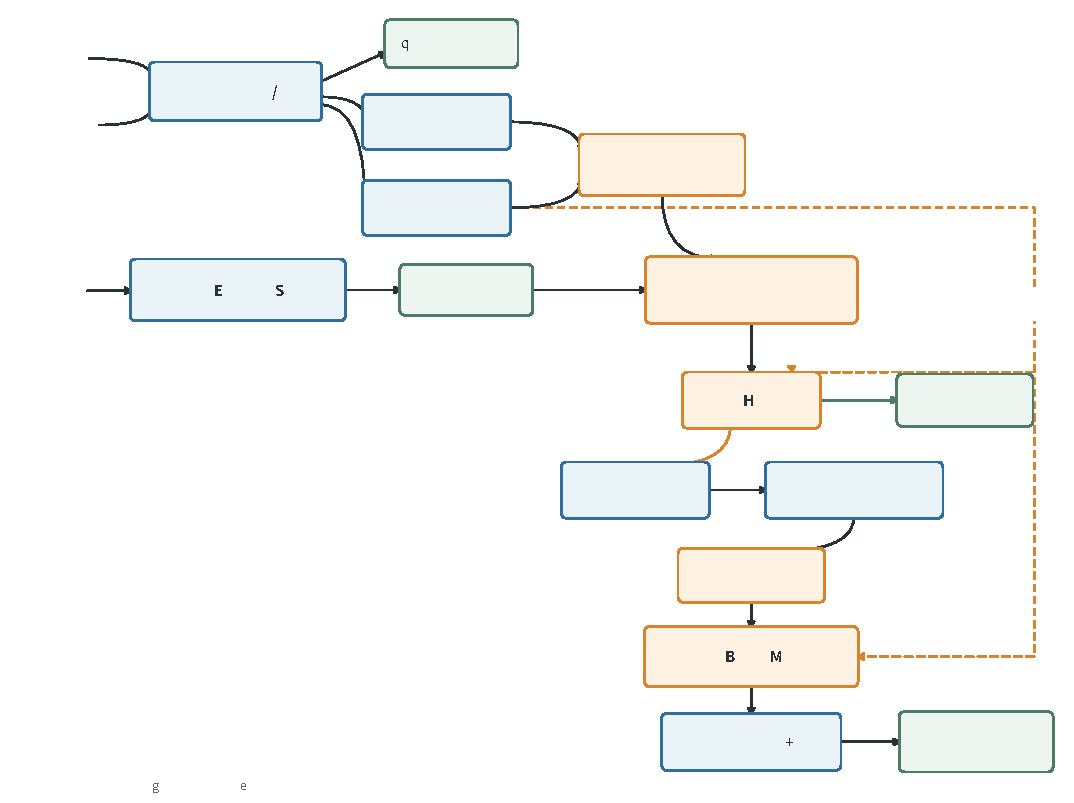
\includegraphics[width=0.96\textwidth]{figures/framework.pdf}%
  }{%
    \missingfigure{总体框架图待绘图任务生成：\texttt{figures/framework.pdf}}%
  }
  \caption{基于正常模板与多模态验证器的 PCB 缺陷检测结果复核总体框架。基础检测器与模板差异模块产生双来源候选。复检门选择调用对象，接受门和安全规则约束修改动作。类别感知融合输出检测结果与审计日志。}
  \label{fig:framework}
\end{figure*}

统一候选先经过复检门。低风险 DET 或 BOTH 候选沿用检测器结果，低风险 DIFF 候选默认拒绝。高风险且位于调用预算内的候选才构造 A2 三面板证据卡。三个面板分别是当前候选紧裁剪、正常模板同位置紧裁剪和带候选框的更大上下文。外观差异图与拓扑差异图不进入证据卡。外观与结构分析用于提出 $C_{\mathrm{diff}}$，八维拓扑向量作为复检门和接受门的候选特征。第~\ref{sec:candidates} 节给出这一输入分工的设计与实证依据。

多模态验证器结合 A2 证据卡与封闭知识 $K$，输出缺陷存在性、预测类别、参考可靠性和固定原因码。系统比较该判断、候选来源与检测器结果，再映射为六种动作之一。修改类动作继续经过接受门、配准质量阈值和安全规则。未获接受的提议动作回退到默认处理。M11 执行动作并消解重复框，输出最终检测集合和审计记录。

\subsection{模块划分与职责}

表~\ref{tab:modules} 列出 M0 至 M11 的输入、输出与职责。模块边界按照可复现的数据流划分，差异候选、证据卡和门控特征各自承担单一功能。

\begin{table*}[t]
  \centering
  \caption{EviGate-PCB 十二个模块的职责划分}
  \label{tab:modules}
  \small
  \setlength{\tabcolsep}{4pt}
  \begin{tabular}{@{}p{0.14\textwidth}p{0.22\textwidth}p{0.22\textwidth}p{0.36\textwidth}@{}}
    \toprule
    模块 & 输入 & 输出 & 职责 \\
    \midrule
    M0 基础检测器 & 待检图像 $I$ & 框、类别、校准置信度组成的 $C_{\mathrm{det}}$ & 快速提供具有类别语义的初始检测候选，不承担模板比较。 \\
    M1 配准与光度归一 & $I$、正常模板 $R$ & 对齐模板、配准质量 $q_{\mathrm{reg}}$ & 统一几何坐标和亮度尺度。量化正常模板对齐是否可靠，为破坏性动作提供降级依据。 \\
    M2 外观差异 & $I$、对齐模板 & 外观差异图 $M_{\mathrm{app}}$ 与区域统计 & 描述材料增减和灰度变化。仅服务于差异候选与门控特征，不作为 A2 证据卡面板。 \\
    M3 结构差异 & 对齐后的图像对 & 结构差异图 $M_{\mathrm{topo}}$、八维拓扑向量 & 计算容差感知的连通性变化。差异图不进入证据卡，拓扑向量作为门控特征。 \\
    M4 差异候选生成 & $M_{\mathrm{app}}$、$M_{\mathrm{topo}}$ 与质量信息 & $C_{\mathrm{diff}}$ & 对差异区域阈值化、过滤和成框，提出可用于恢复漏检的候选假设。 \\
    M5 候选融合 & $C_{\mathrm{det}}$、$C_{\mathrm{diff}}$ & 统一候选 $C$ 与来源标记 & 合并空间一致的候选，标记 DET、DIFF 或 BOTH，并保留动作所需的原框信息。 \\
    M6 复检门 & 检测、差异、拓扑、来源及 $q_{\mathrm{reg}}$ 等候选特征 & 复检风险分数与调用决策 & 在预算内定位更可能被纠正的候选，决定是否调用多模态验证器。 \\
    M7 A2 证据卡 & 高风险候选、$I$、对齐模板 & 三面板视觉证据 & 生成当前紧裁剪、模板紧裁剪和更大上下文，保持对应位置和缩放一致。 \\
    M8 多模态验证器独立判断 & A2 证据卡、封闭缺陷知识 $K$ & 固定 JSON 视觉判断 & 在候选范围内判断缺陷存在性和类别。不自由生成框，不直接执行系统动作。 \\
    M9 动作映射 & 验证器输出、候选来源、检测器结果 & 六类提议动作 & 在模型外比较独立判断与原检测。把结论映射为 keep、remove、relabel、add、reject 或 defer。 \\
    M10 接受门与安全规则 & 候选证据、提议动作、$q_{\mathrm{reg}}$ & 执行或回退决策 & 估计修改是否产生正效用。以动作阈值、配准约束和合法性规则减少有害修正。 \\
    M11 最终融合 & 全部已接受动作与默认结果 & 最终框集合、审计日志 & 执行动作并进行类别感知 NMS，记录候选来源、验证器输出、门控分数及最终决策。 \\
    \bottomrule
  \end{tabular}
\end{table*}

M0 至 M5 确定系统的可复核范围，双来源设计将漏检恢复纳入候选空间。M6 选择调用对象，M7 构造验证输入，M8 输出独立判断。M9 和 M10 决定提议动作是否可以改变结果。第 4 章展开 M1 至 M5，并将 M7 与候选几何一并说明；第 5 章展开 M6、M8、M9 和 M10。M11 的执行规则如下。

\subsection{最终融合与审计（M11）}
\label{subsec:final-fusion}

M11 以基础检测结果为默认集合，只执行通过 M10 的修改类动作。\texttt{remove} 删除对应的检测器原框。\texttt{relabel} 只更新该原框的类别。\texttt{add} 加入 DIFF 候选已有的边界框。\texttt{keep}、\texttt{reject} 和未获接受的提议动作不改变默认集合。\texttt{defer} 在自动评价中同样沿用默认结果，并在审计记录中标为待人工处理。第~\ref{sec:gating} 节的动作合法性、配准质量阈值和回退规则先于本模块执行。

动作执行后，M11 采用 IoU 阈值为 $0.5$ 的类别感知 NMS。同类别重叠框按最终分数降序保留，异类别框不互相抑制。该次序构成同类别冲突的优先级：原有或改类框沿用检测器校准分数，新增框使用接受门概率。删除动作不产生分数，改类动作不改变框坐标。系统不把验证器的文本置信度直接写入检测分数。

每条候选审计记录包含图像与候选标识、来源标记、复检分数与调用状态。记录还包含多模态验证器的结构化输出、提议动作、接受概率和动作执行状态。候选标识可关联 $q_{\mathrm{reg}}$、候选几何和其他门控特征。最终输出另行记录边界框、类别和分数。审计记录据此区分未调用、未接受与已执行三种状态。
